\section{Separating candidate order from answer-code assignment}
\label{sec:codebook}
The legal reversal in Section~\ref{sec:natural-domains} is a useful stress
test, but it is not a single-factor manipulation for the two code-likelihood
LLM adapters: reversing the serialized candidates also changes which
semantic label is assigned to each answer token. We therefore completed a
factorial follow-up on the \emph{same} 144 ContractNLI cases from 91 source
contracts. The original and joint-reversal outputs are reused by hash; two
missing cells reverse only display order or only label-to-code assignment.
The state, option meanings, gold label, model weights and adapter are fixed.
Before inference, the four rendered messages and code maps were frozen and
the reused cells were checked against their historical tokenized-prompt
hashes. A transparent corrective amendment aligned the new inference batch
size to the historical four after an initial batch-eight pilot had already
been inspected; both pilots and all raw outputs remain available. This is a
follow-up diagnostic of these two pinned model--adapter pairs, not a wholly
prospective four-cell test or an intervention on legal reasoning itself.

\begin{figure}[!ht]
\centering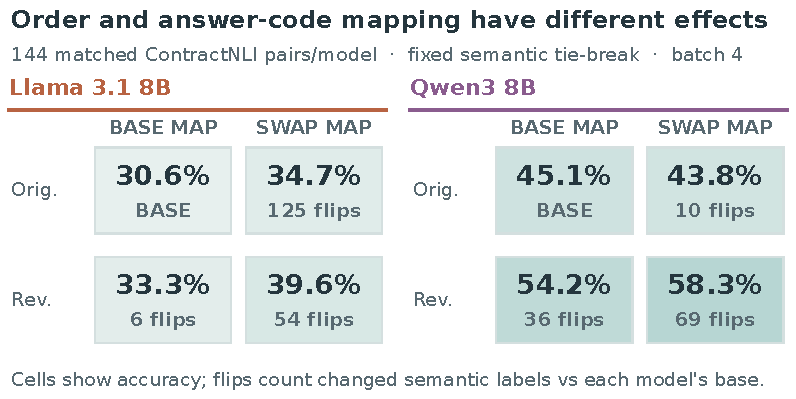
\includegraphics[width=.99\linewidth]{figures/fig_domain_codebook_main.pdf}
\caption{Orthogonal ContractNLI candidate-rendering diagnostic for Llama 3.1
8B and Qwen3 8B ($n=144$ matched document--hypothesis cases/model). Columns
change semantic label-to-code assignment; rows change serialized display
order. Cell accuracy and prediction switches from base use a \emph{common
semantic tie-break} for the 2$\times$2 comparison; this is a labeled post-hoc
sensitivity, not a replacement for the historical native outputs. All cells
are evaluated at historical batch size four; intervals in the text resample
the 91 contracts. The source sample is deliberately class-balanced.}
\label{fig:domain-codebook}
\end{figure}

Figure~\ref{fig:domain-codebook} shows the common-tie comparison. The native
recorded accuracy grid (base, display-only, code-only, both) is
$44,48,50,59$ of 144 for Llama and $65,78,63,83$ for Qwen; all 1,152
cell decisions are valid. Yet the single-factor \emph{prediction} transitions
have nearly opposite geometry. Changing only the answer-code mapping flips
125 Llama labels (86.8\%; contract-cluster 95\% interval [81.1, 92.1]) but
only 10 Qwen labels (6.9\%; [2.8, 11.6]); changing only display order flips
6 Llama labels (4.2\%; [1.4, 7.6]) but 36 Qwen labels (25.0\%; [18.1,
32.2]). The selected code itself reveals why these are not equivalent
perturbations: Llama selects token A in 138/144 base and 131/144 code-only
cases despite the remapping, whereas Qwen shifts from token C in 122/144
base cases to token A in 126/144 code-only cases while mostly retaining its
\emph{semantic} answers. This is evidence of distinct interface coupling in
the two implementations, not a general property of either model family.

There is a third interface degree of freedom: the historical joint-reversal
question also reverses the decoder's first-maximum tie priority. Exact BF16
top-logit ties occur in Llama's base/display/code/both cells $4/0/9/12$
times and Qwen's $0/4/0/5$ times. Re-decoding stored probabilities with
one fixed semantic priority (entailment, contradiction, not-mentioned)
changes only the historical joint cell: Llama $59\to57$ correct and
$66\to54$ base-to-joint flips; Qwen $83\to84$ correct and $64\to69$ flips.
We retain the native counts above for reproducibility, but interpret the
factorial grid only under this common, explicitly post-hoc tie rule.
Under that convention, the joint accuracy effects are $+9.0$ percentage
points for Llama (paired contract-cluster interval $[+2.1,+16.1]$) and
$+13.2$ for Qwen ($[+4.4,+21.4]$). Their difference-in-differences
interactions are $+2.1$ ($[-7.0,+10.8]$) and $+5.6$ points
($[-2.1,+13.0]$), respectively; these intervals do not resolve an
interaction. The original exact-repeat output has zero prediction changes
in either model. Conversely, the batch-eight pilot changes three Qwen
display-only predictions versus the matched-batch result, reinforcing why
batch shape cannot be quietly varied. All intervals describe this selected,
balanced, length-capped legal sample, not ContractNLI's natural test
distribution or system-level legal competence.
\FloatBarrier
